\documentclass[a4paper]{article}

\usepackage[brazilian]{babel}
\usepackage[utf8x]{inputenc}
\usepackage[T1]{fontenc}

\usepackage{listings}
\usepackage{pythonhighlight}

%% Useful packages
\usepackage{amsmath}
\usepackage{graphicx}
\usepackage[colorinlistoftodos]{todonotes}
\usepackage[colorlinks=true, allcolors=blue]{hyperref}

\usepackage{mathrsfs}
\usepackage{amssymb}



%opening
\title{Relatório do Projeto 1}
\author{Daniel Moreira Cestari - 5746193}

\begin{document}

\maketitle

\section{Introdução}

O objetivo do Projeto 1 é o desenvolvimento de uma malha passados alguns parâmetros aplicando os conceitos visto até o momento.

A especificação do projeto pede para gerar uma malha dados, uma distância $D$ entre um círculo de raio $R$ e a borda esquerda do domínio retangular, o domínio tem comprimento $L$ e deve ser dividido em $k$ partições. Sendo que, uma dessas partições necessariamente precisa dividir o círculo em dois. O círculo deve estar centrado no domínio em termos da coordenada vertical. Também é pedido para refinar a malha ao redor do círculo e no centro do domínio à direita do círculo.

A maneira de como o círculo é gerado, como as partições e o refinamento são feitos não estão definidos, sendo livre a escolha.


\section{Implementação}

Nesta seção é apresentada a implementação do código, e o porque de determinadas escolhas.

Basicamente o código está dividido em 3 partes:
\begin{itemize}
	\item \textbf{Geração da curva e domínio}: Nesta etapa é gerada a curva e os limites do domínio baseado nos parâmetros passados. Também é possível ler uma curva de um arquivo ou passar uma função que gere outra curva, tornando a implementação mais genérica.
	
	\item \textbf{Particionamento do domínio e determinação dos bordos}: Basicamente o particionamento do domínio tem apenas duas restrições, dividir a curva no meio e realizar um número $k+1$ de partições ($k$ é o parâmetro passado que determina quantos pontos de quebra o eixo $x$ tem).
	Foram implementadas duas maneiras de determinação dos bordos, chamadas de heurística 1 e 2.
	
	\item \textbf{Geração da malha}: Esta é a única etapa que utiliza código já implementado dos exercícios práticos. Após as várias partições serem geradas, cada uma têm sua malha gerada resolvendo a equação de \textit{Poisson} e ao final são unidas em uma única malha.
	
\end{itemize}

A seguir, cada etapa será descrita com mais detalhes.


\subsection{Geração da curva e domínio}

A geração da curva, no caso um círculo, é realizada por uma função \textit{circle} que recebe 3 parâmetros. Abaixo é exibido o trecho do código com a função.

%%%%%%%%%%%%%%%%%%%%
% def circle
\inputpython{project1.py}{7}{19}
%%%%%%%%%%%%%%%%%%%%

A convenção adotada na geração da curva é começar do ponto mais a direita em $x$ e seguir o sentido anti-horário.
Uma alternativa à geração do círculo, é a leitura de uma curva em arquivo, como o arquivo \textit{naca012.txt} já utilizado em um exercício prático, ou passar uma função que gere outra curva.

%%%%%%%%%%%%%%%%%%%%
% def generate_curve
\inputpython{project1.py}{24}{74}
%%%%%%%%%%%%%%%%%%%%


Na \textit{docstring} é apresentada uma descrição geral da função e de cada parâmetro.
A função \textit{generate\_curve} retorna um dicionário com os pontos que definem o domínio e a curva.


\subsection{Particionamento do domínio e determinação dos bordos}

A função \textit{partitionate\_domain} chama das funções que realizam o particionamento e determinação dos bordos, \textit{heuristic\_1} e \textit{heuristic\_2}. Para a reutilização do código que resolve a equação de \textit{Poisson} cada partição é salva em arquivo, e essa função que salva cada partição em arquivo.
Abaixo é mostrada a função.

%%%%%%%%%%%%%%%%%%%%
% def partitionate_domain
\inputpython{project1.py}{483}{517}
%%%%%%%%%%%%%%%%%%%%

A diferença entre as duas heurísticas está na divisão feita sobre as partições que contém o círculo.

A primeira heurística (função \textit{heuristic\_1}), na partição do círculo, define o bordo de cima como a parte de cima do domínio mais a reta vertical até chegar ao círculo, e o mesmo princípio para o bordo de baixo, seguindo o sentido da esquerda para a direita. Os bordos da esquerda e direita são definidos pela reta vertical e pela curva, dependendo se a partição está a direita ou a esquerda da curva, e seguindo o sentido de baixo para cima.
As figuras \ref{fig:heuristic1_top1} e \ref{fig:heuristic1_top2} mostram as malhas geradas pela heurística 1 nas partições do círculo. As cores definem os bordos, azul bordo de cima, laranja bordo de baixo, verde bordo da esquerda, e vermelho bordo da direita.


 \begin{figure}[h]
 	\centering
 	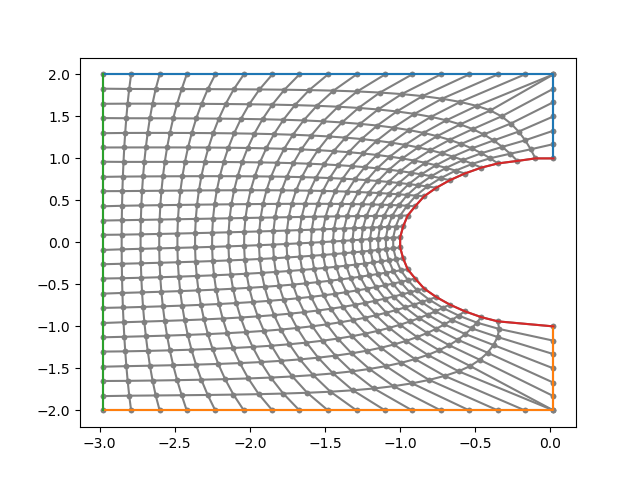
\includegraphics[width=1.0\textwidth]{heuristica_1_50pts_top1.png}
 	\label{fig:heuristic1_top1} 
 	\caption[caption]{Malha gerada pela heurística 1 na primeira metade do círculo}
 \end{figure}


 \begin{figure}[h]
	\centering
	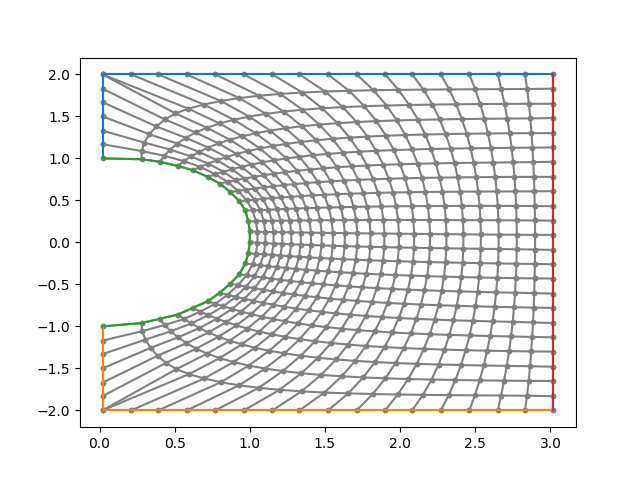
\includegraphics[width=1.0\textwidth]{heuristica_1_50pts_top2.png}
	\label{fig:heuristic1_top2} 
	\caption[caption]{Malha gerada pela heurística 1 na segunda metade do círculo}
\end{figure}


%%%%%%%%%%%%%%%%%%%%
% def heuristic_1
\inputpython{project1.py}{77}{239}
%%%%%%%%%%%%%%%%%%%%





A heurística 2 difere da 1, na sua definição dos bordos sobre a partição da curva. Neste caso, a divisão é feita seguindo o lado, se lado em questão está a esquerda então é o bordo esquerdo, se está a direita é o bordo direito, se está acima é o de cima e se está abaixo o de baixo.
As figuras \ref{fig:heuristic2_top1} e \ref{fig:heuristic2_top2} mostram malhas geradas utilizando a heurística 2, as cores têm o mesmo significado que o relatado na heurística 1.

\begin{figure}[h]
	\centering
	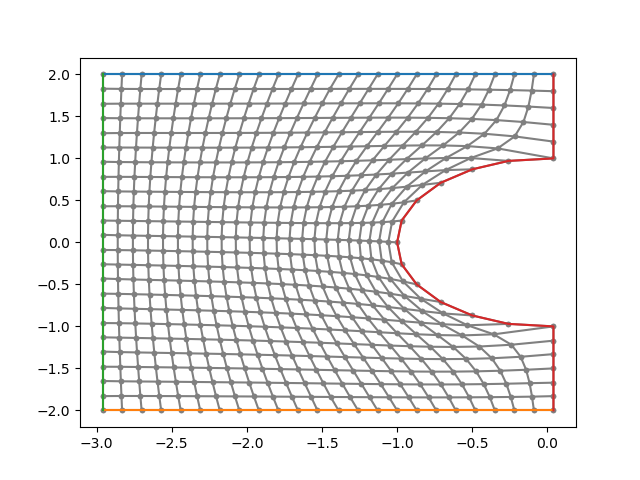
\includegraphics[width=1.0\textwidth]{heuristica_2_25pts_top1.png}
	\label{fig:heuristic2_top1} 
	\caption[caption]{Malha gerada pela heurística 2 na primeira metade do círculo}
\end{figure}


\begin{figure}[h]
	\centering
	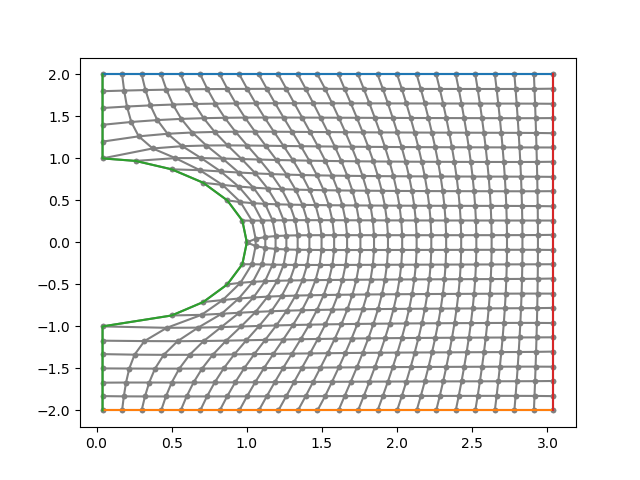
\includegraphics[width=1.0\textwidth]{heuristica_2_25pts_top2.png}
	\label{fig:heuristic2_top2} 
	\caption[caption]{Malha gerada pela heurística 2 na segunda metade do círculo}
\end{figure}


%%%%%%%%%%%%%%%%%%%%
% def heuristic_2
\inputpython{project1.py}{256}{480}
%%%%%%%%%%%%%%%%%%%%


\subsection{Geração da malha}

A função que gera a malha chama as funções que criam o domínio e o particionam, e depois resolve a equação de \textit{Poisson} em cada partição individualmente.

Essa é a principal função que chama todas as outras necessárias, e por isso é cheia de parâmetros. Todos descritos na \textit{docstring}, basicamente juntou todos os parâmetros das funções anteriores mais os parâmetros relativos ao refinamento da malha.

Abaixo é apresentada a função \textit{generate\_grid}.

%%%%%%%%%%%%%%%%%%%%
% def generate_grid
\inputpython{project1.py}{529}{574}
%%%%%%%%%%%%%%%%%%%%




\section{Resultados}

% mostrar os vários processo
as duas heurísticas com e sem refinamento
depois o aerofólio nas duas heurísticas, com e sem refinamento também







\end{document}
